\documentclass[tikz,border=5pt]{standalone}
\usepackage{amsmath}
\usetikzlibrary{angles}

\begin{document}
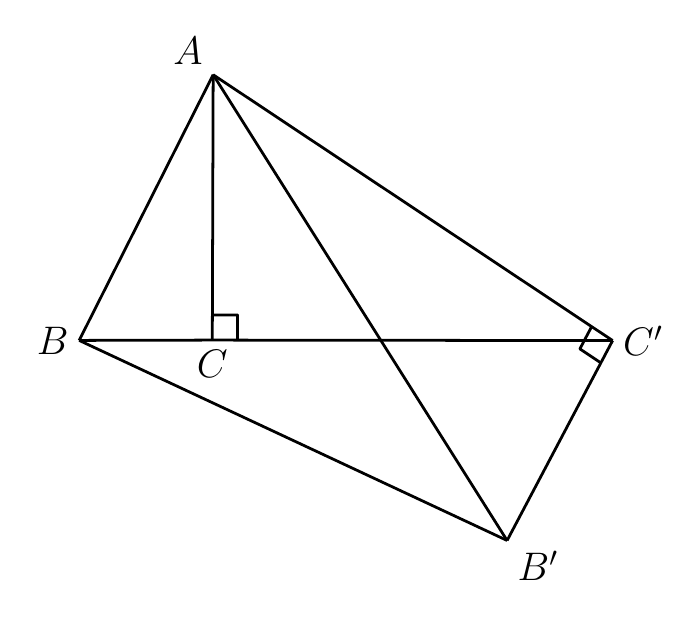
\begin{tikzpicture}[line width=1.0pt, line join=round]
\coordinate (A) at (-1.774,2.984);
\coordinate (B) at (-3.476,-0.390);
\coordinate (C) at (-1.785,-0.386);



  
  \coordinate (Cp) at (3.299,-0.392);
  \coordinate (Bp) at (1.959,-2.931);

  
  \draw (A) -- (B);
  \draw (A) -- (C);
  \draw (B) -- (C) -- (Cp);   
  \draw (A) -- (Cp);
  \draw (Cp) -- (Bp);
  \draw (B) -- (Bp);
  \draw (A) -- (Bp);

  
  \draw pic[draw, angle radius=0.320cm] {right angle=A--C--Cp};
  \draw pic[draw, angle radius=0.320cm] {right angle=A--Cp--Bp};

  
  \node[font=\fontsize{14.5}{17.4}\selectfont, above left] at (A) {$A$};
  \node[font=\fontsize{14.5}{17.4}\selectfont, left] at (B) {$B$};
  \node[font=\fontsize{14.5}{17.4}\selectfont, below] at (C) {$C$};
  \node[font=\fontsize{14.5}{17.4}\selectfont, right] at (Cp) {$C'$};
  \node[font=\fontsize{14.5}{17.4}\selectfont, below right] at (Bp) {$B'$};
\end{tikzpicture}
\end{document}